% !TeX root = ../main.tex
\section{Design of Compiler}
The compiler is composed of three primary parts, which is explained in the following sections.
The explanation covers both code snippets of the compiler and reasoning behind development decisions.
However, it is also quite important to address the decisions regarding each component on a larger scale, each phase of the compilation process, and to introduce the components of the compiler before they are explained in depth.
\begin{figure}[H]
	\centering
	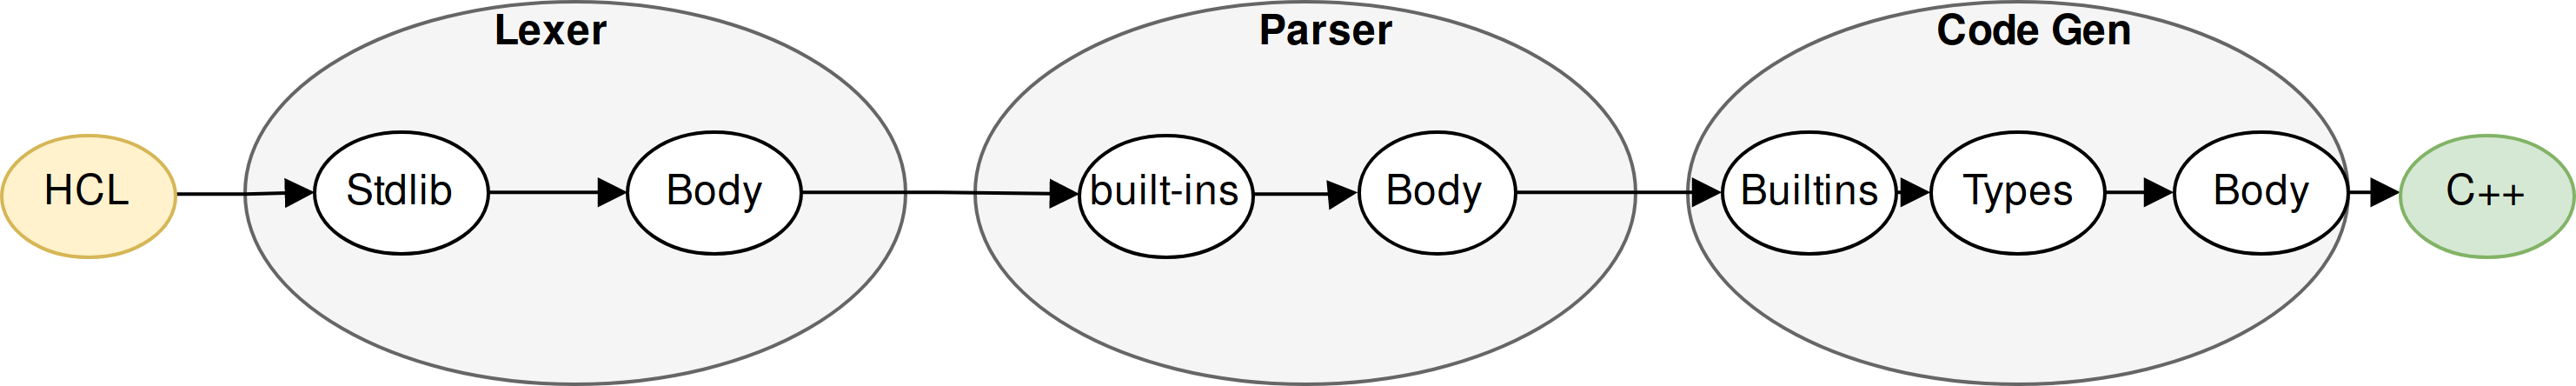
\includegraphics[width=\textwidth]{4.Solution/images/compiler_process.png}
	\caption{The three major components of the compiler}
	\label{fig:compilerProcess}
\end{figure}


The compiler is composed of a lexer, a parser, and a code generator, as seen in figure \ref{fig:compilerProcess}.
The lexer generates a token stream from a text stream, which is fed into the parser, which then builds an AST based on the tokens.
The abstract syntax tree is then processed by the code generator, which outputs code in our output language, \texttt{C++}.

Some compilers are built with an isolated type checker.
However, as the HCL language only allows predefined types and has a relatively simple structure, the type checking happens as part of the parser.

Checking the validity of identifiers also happens in the parser.
This means that the parser is the largest part of the compiler.
Type checking is done with a symbol table, which is composed of layers that are pushed and popped when entering and leaving a scope.
 
As the HCL language has built-in functions, these are hard-coded into the parser, and are added to the symbol-table as the first part of the parsing procedure.

Other compilers often have an optimization phase, but this has been deemed irrelevant as the output language has to go through another compiler which most likely has an optimization phase of its own. 
With this in mind, more energy has been put into creating a good parser and code generator than optimizing the efficiency of the output program.
